\documentclass{article}
\usepackage[left=2cm,right=2cm,top=1cm,bottom=1cm,a3paper]{geometry}
\usepackage{pgfplots}
\usepackage{parskip}
\usepackage{caption}
\usepackage{multicol}
\usepackage{wrapfig}
\usepackage[]{mathtools}
\usepackage{float}
\restylefloat{table}

\setlength{\parindent}{0mm}

\pgfplotsset{compat=1.15}

\newcommand{\cia}[1]{\resizebox{\textwidth}{!}{\input{#1}}}
\newcommand{\ciapdf}[1]{\vspace*{-\parskip}\begin{center}\resizebox{0.75\textwidth}{!}{\includegraphics[width=0.75\textwidth]{#1}}\end{center}}
\newcommand{\halfhalf}[2]{\begin{multicols}{2}\includegraphics[width=0.5\textwidth]{#1} \includegraphics[width=0.5\textwidth]{#2}\end{multicols}}

\begin{document}

\title{Assignment one: supervised learning}
\author{Lin Zhao (16010906)}
\date{\today}
\maketitle

\newpage

\section*{Task 1}

\subsection*{Introduction}

The dataset used for this task is from Schularick and Taylor(2012,
``Credit Booms Gone Bust''). It is an annual dataset covering 14
countries and 140 years. Among the variables they collected, the most
important one is the yearly aggregate bank loans, which is 
the main soure of predictive power. The variable of interest is the
CrisisST which take a value of 1 when there is a financial crisis and 0
otherwise.

Following the guidance of Schularick and Talor(2012), I explored the
relationships between several macro variables within two
eras of finance capitalism, tested the predictive power of different
macro variables, and compared predictive power of different supervised
learning methods. The last part of above is also inspired by the
Fricke(2017, Financial Crisis Prediction: A Model Comparison``). 

The methods used are logistic regression, classification
tree, classification forest, and SVM. The major criteria
used here is area under receiver operating curve. The secondary creteria
is confusion matrix. The major validation method is the modified cross
validation method  as mentioned in the Fricke paper that takes time order into
consideration.

\subsection*{Data description and cleaning}

To explore the changing features between two eras, firstly I created
variables of interest: credit to GDP ratio, bank asset to GDP ratio,
money to GDP ratio, credit to money ratio, and bank asset to money
ratio. To see the distinctive trends in different historical periods, I
regroup the whole dataset by years and take mean value of each variable
each year. Ploting mean values of the ratios above against time, I
recovered Figure 1 and 2 in Schularick and Taylor(2012).

Figure 1 shows that bank loans, bank asset and broad money supply remain
steady related to the size of economy representing by GDP,
before the WW2 period. After the war, the money to GDP ratio stays flat
while the other two start to increase dramatically. In figure 2 we
can see that the loan to money ratio and bank asset to money ratio start
to take off after the distruction of WW2 implying that credit start to
grow faster than broad money supply and no steady relationship between
the too can be found in this period.

\ciapdf{Figure_2.pdf}

\begin{quote}
Figure 1: Aggregates relative to GDP (year effects)
\end{quote}

\ciapdf{Figure_1.pdf}

\begin{quote}
Figure 2: Aggregates relative to broad money (year effects)
\end{quote}

To study financial crisis caused by the internal reasons from economic system,
we need to
exclude the crisis caused by the two world wars. As did in Schularick and
Taylor paper, I excluded the war periods (1914 to 1919 and 1939 to 1947)
and German crisis after WW1(1920 to 1925). Divided the cleaned up
dataset into pre- and post-war periods, I recovered the upper panel of
table 1 in the paper.

\subsubsection*{\centering{}Annual summary statistics pre- and post-war}

\begin{table}[H]
    \begin{center}\begin{tabular}{|l|l|l|l|l|l|}
    \hline
          & credit\_to\_GDP & bankAsset\_to\_GDP & money\_to\_GDP & credit\_to\_money & bank\_asset\_to\_money \\ \hline
          & Pre-war         &                    &                &                   &                        \\ \hline
    count & 685             & 611                & 736            & 662               & 580                    \\ \hline
    mean  & 0.408977        & 0.714051           & 0.533292       & 0.735337          & 1.282481               \\ \hline
    std   & 0.359888        & 0.447337           & 0.207534       & 0.449343          & 0.566104               \\ \hline
          & Post-war        &                    &                &                   &                        \\ \hline
    count & 831             & 828                & 834            & 833               & 831                    \\ \hline
    mean  & 0.546975        & 1.013497           & 0.645801       & 0.838012          & 1.575839               \\ \hline
    std   & 0.423878        & 0.668770           & 0.240497       & 0.494226          & 0.752540               \\ \hline
    \end{tabular}\end{center}
\end{table}

More than half of the countries in the dataset are from
Europe, so I also excluded all the observations in post WW1 period(1920 to
1925) since all the crises happened in
that period could be caused by WW1 rather than economic system. I
only kept the variables that have protentially strong predictive power
according to the results and the robustness test from the paper.

After dropping any row that contains missing value, I have 1433 observations
and 59 out of these are crisis
events.

\subsection*{Supervised learning methods for classification}

\subsubsection*{Logistic regression and choice of explanatory variables}

As defined in Schularick and Taylor paper, I created CPI nomalized bank
loan and take the difference of log values of this variable as the change
of credit environment. This variable will be called credit change. I also
take credit to GDP ratio as one protential
explanatory variable base on robustness test of the paper. This variable
lagged 1 year will be called credit size. After
assign each country for each year its lagged 1 to 5 credit change and credit size, I
sorted the dataset by time to make sure that when fitting a model, it is
not trying to predict 1960s crisis with 1990s' data.

I started the analysis by useing lag 1 to lag 5 credit change to fit a
logistic regression model. The AUC is slightly higher than 0.5 for the whole
dataset and for the pre-war dataset, and significantly higher than 0.5
for the post-war dataset. Since in the paper, lag 2 credit change is the only
lagged variable that
is significant, I also fitted logistic regression with only lag 2 data
and the model fit slightly better for both whole set and pre-war period
in respect of AUC. The change in post-war period is umbiguous and 
credit size seems add predictive power to the post-war period. The lag 2 credit
change is indeed the
main sourece of information.

\subsubsection*{\centering{}In-sample AUC for logistic regression with lag 1 to 5 credit change}

\begin{table}[H]
    \begin{center}\begin{tabular}{|l|l|l|l|}
    \hline
                        & whole set          & pre-war            & post-war           \\ \hline
    without credit size & 0.5861360718870345 & 0.5762987012987013 & 0.7608543417366948 \\ \hline
    with credit size    & 0.5892169448010269 & 0.5892169448010269 & 0.615546218487395 \\ \hline
    \end{tabular}\end{center}
    \caption{in-sample logistic regression trained with whole time period,
    pre-war period and post-war period with lag 1 to 5 credit change as major
    explanatory variable.}
\end{table}

\subsubsection*{\centering{}In-sample AUC for logistic regression with lag 2 credit change}

\begin{table}[H]
    \caption{in-sample logistic regression trained with whole time period,
    pre-war period and post-war period with lag 2 credit change as major
    explanatory variable.}
    \begin{center}\begin{tabular}{|l|l|l|l|}
    \hline
                        & whole set          & pre-war            & post-war           \\ \hline
    without credit size & 0.6373277827336704 & 0.6286424526999033 & 0.697533908754624  \\ \hline
    with credit size    & 0.4518906730102092 & 0.5177922018137459 & 0.7200369913686806 \\ \hline
    \end{tabular}\end{center}
\end{table}

I did a out-of-sample test for the choice of variable using
30\% of the dataset as test set and 70\% as training set.
The results show that model fitted with lag 2 credit change have
significantly better out-of-sample performance than model fitted with
lag 1 to lag 5 and credit size doesn't seem to add predicting
power to the model. The AUC are reported in the following tables.

\subsubsection*{\centering{}Out-of-sample AUC for logistic regression with lag 1 to lag 5 credit change}

\begin{table}[H]
    \caption{out-of-sample logistic regression trained with 70\% of
    each data set and tested on 30\% of data with lag 1 to lag 5
    credit change as major explanatory variable.}
    \begin{center}\begin{tabular}{|l|l|l|l|}
    \hline
                        & whole set          & pre-war            & post-war           \\ \hline
    without credit size & 0.5861360718870345 & 0.5762987012987013 & 0.7608543417366948 \\ \hline
    with credit size    & 0.5892169448010269 & 0.5800865800865801 & 0.615546218487395  \\ \hline
    \end{tabular}\end{center}
\end{table}


\subsubsection*{\centering{}Out-of-sample AUC for logistic regression with lag 2 credit change}

\begin{table}[H]
    \caption{out-of-sample logistic regression trained with 70\% of
    each data set and tested on 30\% of data with lag 2 credit change
    as major explanatory variable.
    }
    \begin{center}\begin{tabular}{|l|l|l|l|}
    \hline
                        & whole set          & pre-war            & post-war           \\ \hline
    without credit size & 0.7370988446726572 & 0.7976190476190476 & 0.7461484593837535 \\ \hline
    with credit size    & 0.531193838254172  & 0.6737012987012987 & 0.6355042016806722 \\ \hline
    \end{tabular}\end{center}
\end{table}

\ciapdf{Figure_4.pdf}
\begin{quote}
Figure 3: out-of-sample AUC of logistic fitted with 70\% of
data as training set and 30\% as testing set. All three periods
fitted with lag 2 credit change only.
\end{quote}

Given result above, I only considered lag 2 credit change and credit
size variables in the rest of this study. This also means all the models
compared here will have
same information as input and thus makes the comparison meaningful.

At last for logistic regression, I did a modified cross validation as
mentioned in the Fricke paper. I divided the wholde dataset in to four
equal folds. First, I use fold one to train and test on fold two. Then I
use fold one and two to train and test on fold three, etc.. The average
AUC is 0.56129 which is higher than 0.5. The reason for divide the
dataset into 4 rather than 5 fold like did in the Fricke paper is that
when the fold is too small, due to the sparseness of crisis events,
there might be only one class in the whole training set or test set.

\subsubsection*{Tree and forest}

Next I fitted the data with a classification tree. With maxmum depth
equals to 3, here are result of in-sample prediction. It is obvious from
the table that credit size add on predictive power for classification
tree at least for in-sample test.

\subsubsection*{\centering{}AUC for classification tree}

\begin{table}[H]
    \caption{
    in-sample classification tree fitted with lag 2 credit change
    as major explanatory variables
    }
    \begin{center}\begin{tabular}{|l|l|l|l|}
    \hline
                        & whole set          & pre-war            & post-war           \\ \hline
    without credit size & 0.6937568143522649 & 0.7030106338903466 & 0.780209617755857  \\ \hline
    with credit size    & 0.7598684210526315 & 0.7878746029553929 & 0.8358199753390876 \\ \hline
    \end{tabular}\end{center}
\end{table}

From the AUC plot we can see that there are much less point on each line
for the tree compared with logistic regression. This is because for
logistic regression, each observation will have its own estimated
probability, but for a tree, the observations belong to the same leaf
will have the same probability.

\ciapdf{Figure_5.pdf}
\begin{quote}
Figure 4: AUC of classification tree fitted with whole time period,
pre-war and post-war period. All three period fitted with lag 2 credit
change and credit size.
\end{quote}

For the choice of maxmum depth, we need a good balance between fully use
all the information and avoid over fitting. To find the maxmum depth
that gives highest AUC for each tree, I performed an analysis with
following steps: 1\textgreater{} for each of whole set, pre-war, and
post-war period, set up a modified cross validation of 5 fold as
mentioned in logistic regression part with certain maxmum depth and
record the average AUC for each model. 2\textgreater{} collect average
AUC of each model for maxmum depth from 2 to 50. 3\textgreater{} plot
the average AUC against maxmum depth for each model and pick up the
depth that coincide with the highest AUC.

\ciapdf{Figure_6.pdf}
\begin{quote}
Figure 5: Average AUC for the whole, pre- and post-war dataset fitted
with and without credit size plot against maxmum depth
\end{quote}

With optimal max-depth 3, 3, 5 respectlly, I fitted 70\% training set of whole period and
pre-war dataset with lag 2 credit change and post-war with lag 2 credit
change and credit size. With 30\% of the total data as a test set, these models show AUC 0.62895,
0.69021 and 0.43697 respectlly.

The dramatically different performance between in-sample and
out-of-sample test is expected and indecates over fitting. Given a high enough
max-depth, classification tree can acheive AUC 1.0 in an in-sample test.
But over fitting will lead to very poor out-of-sample prediction. This
is indicated by the flatening out in the figure above. Two trees with different maxmum depth in the appendex demonstrate
this point.

With exactly same idea, I performed analysis with classification forest
model. The in-sample performance is better than the tree with same
max-depth which in general indicate higher predictive power. However, forest is also
vulnerable to overfitting.

\subsubsection*{\centering{}AUC for classification forest}


\begin{table}[H]
    \caption{in-sample classification forest fitted with lag 2 credit change
    as major explanatory variable.}
    \begin{center}\begin{tabular}{|l|l|l|l|}
    \hline
                        & whole set          & pre-war            & post-war           \\ \hline
    without credit size & 0.7419033105362275 & 0.7823735211526954 & 0.9169852034525278 \\ \hline
    with credit size    & 0.7619994548518189 & 0.8678359342632234 & 0.8669852034525277 \\ \hline
    \end{tabular}\end{center}
\end{table}

\ciapdf{Figure_7.pdf}
\begin{quote}
Figure 6: AUC of classification forest fitted with whole time period,
pre-war and post-war period. First two period fitted with lag 2 credit
change and credit size and post-war fitted with lag 2 credit change
only.
\end{quote}

With optimal max-depth picked up by the same method as in the tree
analysis, datasets are fitted with lag 2 credit change and/or credit
size. Tested with 30\% data in the dataset, the AUC are 0.62426,
0.73593, and 0.71709 for whole, pre-war and post-war data.

Tree and forest learners perform brilliantly in-sample and
are not much more impresive than logistic regression in out-of-sample test. Due
to the adventage of averaging multiple trees, and reduce overfitting and
variance, forest
performs slightly better than tree method.

In both tree and forest analysis, I used gini index and entropy and
there are little difference between the AUC.

\subsubsection*{SVM}

When fitting SVM model with the data, I used two kinds of kernels:
rbf(Gaussion kernel) and sigmoid kernel. The results are both affected
by randomness when fitting the model and sigmoid kernel in general has
better out of sample perfomance. 


\subsection*{A few interesting facts and potential explanations}


When taking a closer look at the results of tree and forest, I found a
few interesting facts. First, for both tree and forest, I found the
results are different when fitting models with exactly same data set and
parameters, indecating randomness in the
fitting precesure. Second, for the
models fitted with both lag 2 credit change and credit size, the average
AUC show fluctuation in the over fitting zone when plotted with maxmum depth.
In the plot of forest,
all models show fluctuation in the over fitting parts but for models
with two explanatory variables, the fluctuations have higher amplitudes.
Last, for some trees and forests, the out
of sample AUC do not drop to 0.5 even in the obviously over fitting
zone.

To answer the first question, one need to identify the souce of
randomness. I found two protential sources for tree and three for
forest by reading the document. One obvious candidate is the random start point when searching
for the optimal arguments to minimize cost function. However, as long as
the problem is convex, the searching reslults should be with in a
relatively small intervel with possible difference due to limited resolution. This
doesn't match the observation. An argument
called max\_features in tree is defined as``The number of features to consider when
looking for the best split(sklearn.tree.DecisionTreeClassifier document
page)''. When fitted with two variables, the model with max
feature setted to 1 shows jumps while model with max features setted to 2 does not. For the forest, there is one extra
source of randomness. To grow multiple trees, the sklearn library
bootstrap observations using random selection with replacement. In both tree
and forest functions from sklearn library, the argument random state controls all the
randomness.

Carrying knowledge mentioned above, I try to decompose the fluctuations.
Fixing random state eliminates fluctuation in
AUC-max-depth plot of both treee and forests. For the forest, I first turn off the max
feature limit, and the resulting plot doesn't show less fluctuation.
Next, I add the limit on max feature and turn off bootstrap, and
this reduced the fluctuation. And eventually, when I turn off both limit
and bootstrap, the fluctuation was almost totally eliminated. These
changes indicates that the
forest fitting is extremely sensitive to the chang of training dataset.
Another interesting observation here is that the AUC of model fitted
with pre-war data and with both credit change and credit size as
explanatory variables dropped below 0.5 benchmark after the limit and
bootstrap was turn off. I cannot explain this change. Relavent plots are in the appendix.

I notice that the model that has
predictive power even when over fitted are models fitted with the whole
dataset. This is ture for both tree and forest analysis(with
randomness turn off in forest). From the plot of AUC of trees fitted
with different datasets, I notice that there is only one point in each
of the three line. This indecates that in the out of sample test, only
one split, presumably the first split take effect, most likely due to
over fitting. The whole set has the largest number of observations, it is likely that
even when over fitted, the first split still has some predictive power. Here
is one exampel of AUC plot when over fitted. This also explains the same
observation in the forest analysis.

\ciapdf{Figure_11.pdf}
\begin{quote}
Figure 7: All three models are fitted with lag 2 credit change and
credit size. These models are fitted with 80\% of dataset and
tested on 20\% of set. To eliminate effect of randomness, the
ramdom state argument was fixed when fit these models.
\end{quote}

\subsection*{Another criteria}

Except for AUC, a few other values from confusion matrix can also be good
criterias for model comparison. In the tables below, I collected some 
out-of-sample results for logistic regression and forest fitted with 70\%
of whole data set regarding confusion matrix. False alarm is defined as
M01 / (M01 + M11), and can be interpreted as when model say crisis, how much
of that are miss classified. Total flag is the percentage of total
observation that has been flagged by the model as crisis.

To capture 10\% of the crisis,
logistic regression need to flag 2\% of the total observation, and 80\%
of those flags are false alarm. On the other hand, forest need only flag
less than 1\% of data and only half of those are false alarm. However,
if the goal is to capture half of the crisis, logistic regression only
need to flag less than 20\% of data with 87\% false alarm while forest
need to flag half of the data point and more than 90\% of the flag are
false alarm. The main idea here is that there is no sigle best criteria
and the criteria selection should be based on the goal of analysis.

\begin{multicols}{2}
\begin{table}[H]
        \caption{Out-of-sample performance for logistic regression based on confusion matrix.
        Logistic regression fitted with 70\% of the whole period and
        tested with 30\% of whole period. Explanatory variable is lag 2
        credit change only. AUC is 0.73709.}
        \begin{center}\begin{tabular}{|l|l|l|l|}
        \hline
         threshold         & sensitiveity        & falseAlarm         & totalFlag            \\ \hline
        0.95845 & 0.05263 & 0.87500              & 0.01865 \\ \hline
        0.95842 & 0.10526 & 0.80000                & 0.02331 \\ \hline
        0.95829 & 0.15789 & 0.80000                & 0.03497  \\ \hline
        0.95817 & 0.21053 & 0.84000               & 0.05828  \\ \hline
        0.95814 & 0.26316  & 0.83333 & 0.06993  \\ \hline
        0.95805 & 0.31579  & 0.86047 & 0.10023  \\ \hline
        0.95801 & 0.36842  & 0.86000               & 0.11655  \\ \hline
        0.95799 & 0.42105 & 0.85185 & 0.12587   \\ \hline
        0.95796 & 0.47368 & 0.85714 & 0.14685  \\ \hline
        0.95793 & 0.52632  & 0.87179 & 0.18182  \\ \hline
        0.95791 & 0.57895  & 0.88172 & 0.21678  \\ \hline
        0.95790 & 0.63158   & 0.88119 & 0.23543  \\ \hline
        0.95789 & 0.68421  & 0.88288 & 0.25874  \\ \hline
        0.95786 & 0.73684  & 0.89313 & 0.30536  \\ \hline
        0.95773 & 0.78947  & 0.92823 & 0.48718  \\ \hline
        0.95767 & 0.84211  & 0.93701  & 0.59207   \\ \hline
        0.95764   & 0.89474  & 0.93885 & 0.64802   \\ \hline
        0.95759 & 0.94737  & 0.94098  & 0.71096    \\ \hline
        0.95745 & 1.00000                 & 0.95000               & 0.88578   \\ \hline
        \end{tabular}\end{center}
\end{table}

\begin{table}[H]
        \caption{Out-of-sample performance for forest based on confusion matrix. Forest fitted with 70\% of the whole period and tested on
        30\% of the whole period. Variable is lag 2 credit change only,
        max depth is 3. The AUC of this model is 0.67079.}

    \begin{center}\begin{tabular}{|l|l|l|l|}
    \hline
     threshold           & sensitiveity        & falseAlarm         & totalFlag            \\ \hline
    0.31088  & 0.05263 & 0.00000                & 0.00233 \\ \hline
    0.15587  & 0.10526 & 0.50000                & 0.00932 \\ \hline
    0.05381   & 0.15789 & 0.90909 & 0.07692  \\ \hline
    0.04785 & 0.36842  & 0.89394 & 0.15385  \\ \hline
    0.04160  & 0.73684  & 0.93665 & 0.51515   \\ \hline
    0.03808  & 0.84211  & 0.93822 & 0.60373   \\ \hline
    0.03177  & 0.89474  & 0.93885 & 0.64802   \\ \hline
    0.01070 & 0.94737  & 0.95000               & 0.83916   \\ \hline
    0.00829  & 1.00000                 & 0.95571 & 1.00000                  \\ \hline
    \end{tabular}\end{center}
\end{table}
\end{multicols}

\subsection*{Conclusion and potential further questions to answer}

In this study, I implemented
a few supervised learning models on the data. The major predicting
power lies in lag 2 credit change and this conclusion alines with
Schularick and Taylor paper. Predictive power of models are much stronger in sample. This confirms the result of Fricke
paper. Tree and forest are particularly
vulnarable to over fitting thus require carefully picked parameters like
maxmum depth or maxmum number of leaves. They are also quite sensitive
to the change of training set. Another issue for
tree and forest is that when there is a dominating class in the training
data, the model generated could be biasd. This issue can be reduced by
balance the data prior fitting or assign similar weight to different
classes. However, these are not explored in this report and can be
interesting topic for futher study. Since forest shows great protential
to predict crisis, and machine learning methods are not widly use in
economic research, solving this issue could have practical meaning. All
the models tested in this report show some level of predictive power.
However, there is no single standard to judge which is the best model.
The selecting criteria strongly depends on the purpose of the analysis
and different models may have adventages in different tasks.

\begin{thebibliography}{9}
\bibitem{booms} 
Moritz Schularick \& Alan M. Taylor
\textit{Credit Booms Gone Bust: Monetary Policy, Leverage Cycles, and Financial Crisis, 1870-2008}.

\bibitem{fcp} 
Daniel Fricke
\textit{Financial Crisis Prediction: A Model Comparison}.
\end{thebibliography}

\section*{Appendix}

Figure 8: nomal depth tree

\ciapdf{app_normaldepth.pdf}

Figure 9: over fitting tree 

\vspace*{-\parskip}\resizebox{\textwidth}{!}{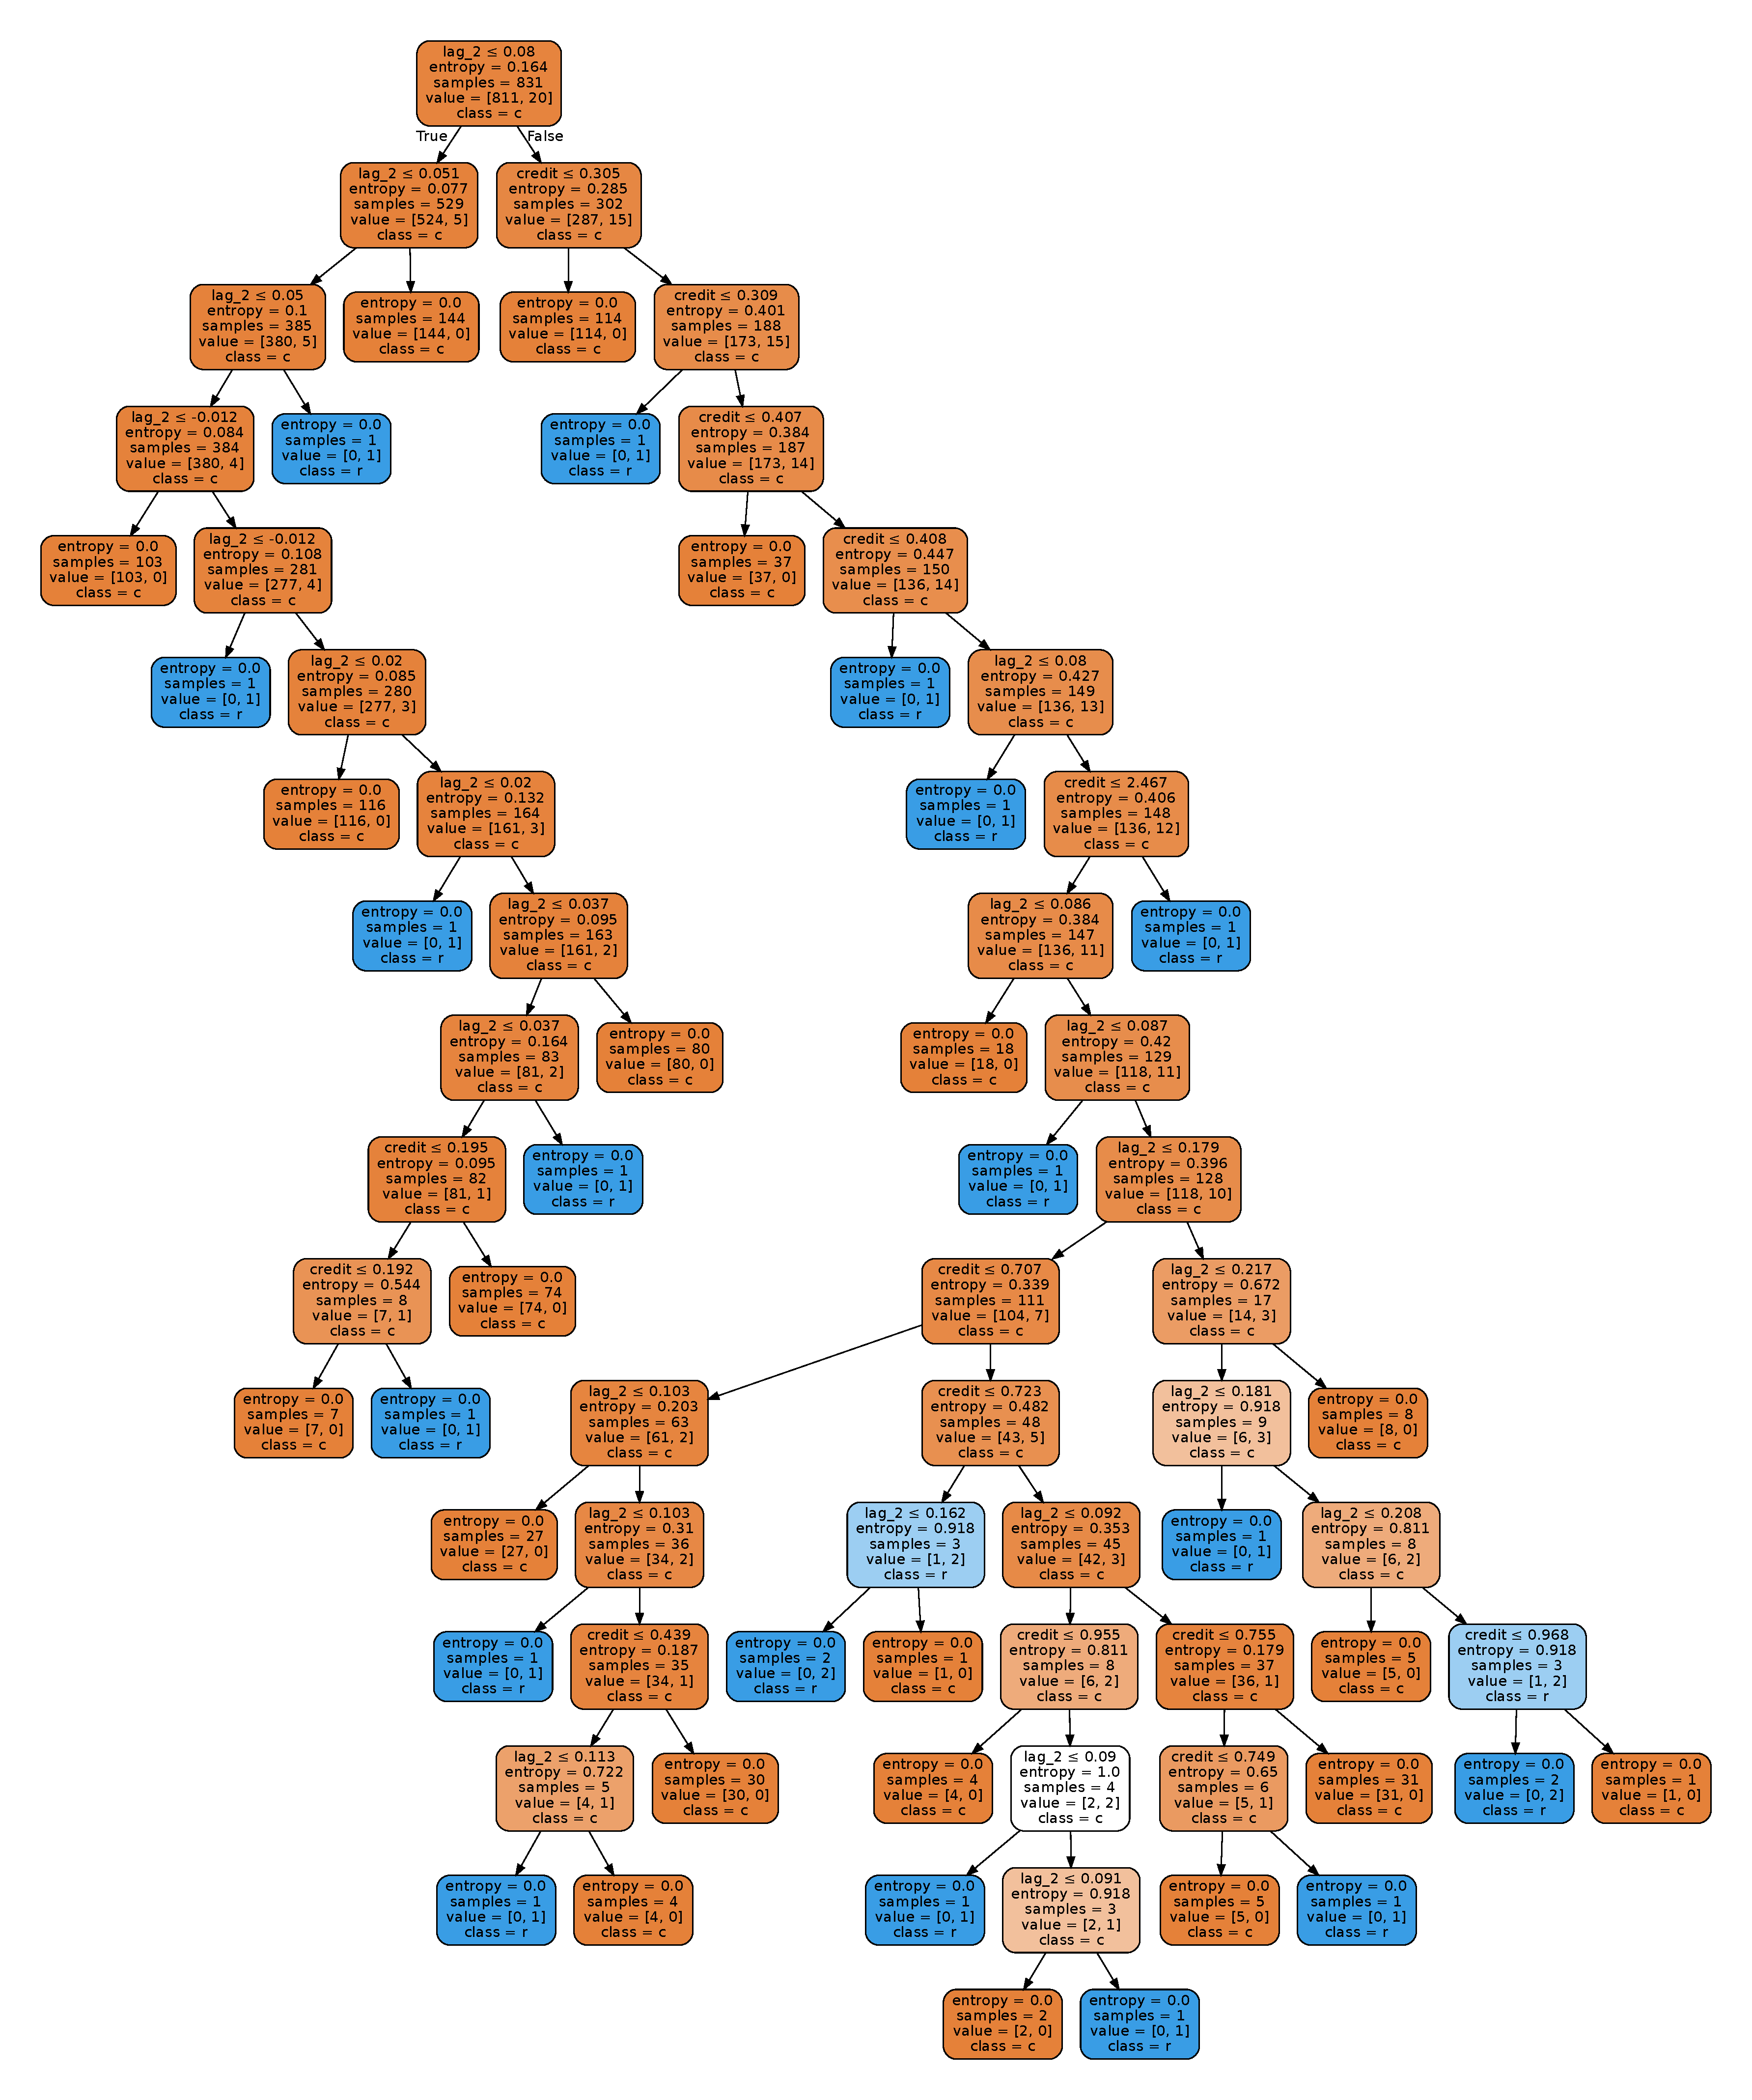
\includegraphics{app_overfitting.pdf}}

Figure 10:
different trees generated by same data with limited max feature. We can see
there is a tie in the cost function values.

\ciapdf{app_samedata_1.pdf}

\ciapdf{app_samedata_2.pdf}

\ciapdf{Figure_8.pdf}
\begin{quote}
Figure 11: The maxmum feature is limited and bootstrap is on, this is
exactly the same plot used to choose optimal depth. We can see a lot of
fluctuation here and at least three AUC do not approach 0.5 benchmark.
\end{quote}

\ciapdf{Figure_9.pdf}
\begin{quote}
Figure 12: The maxmum feature is limited and bootstrap is off, and we can
see that fluctuation is reduced.
\end{quote}

\ciapdf{Figure_10.pdf}
\begin{quote}
Figure 13: The maxmum feature is unlimited and bootstrap is off, and we
can see dramatical reduce of fluctuation and only two lines do not
approach 0.5 benchmark.
\end{quote}

\section*{Task 2}

\subsection*{Introduction}

Markovitz pertfolio theory has always be a classic. However it is known that
the optimal portfolio is not stable bringing issue on frequently rebalancing
for investors. Following the lead of Fastrich, Paterlini, and Winker (Constructing
optimal sparse portfolios using regularization methods, 2014), this study
try to find global minimum variance portfolio under regularizations thus stablize
the portfolio choice and reducing the rebalancing problem.

The regularizations used in this study are Lasso and Ridge. Resulting global
minimum variance portfolios has lower variance than Markovitz portfolios and
therefore confirmed the results from paper montioned above.

\subsection*{Data description and cleaning}

The data used is French 48 industry portfolios daily data. After comparing variance
of each industry and of the whole dataset, I choose to use equal weighted data
since it has higher variance and hopefully the different among regularizations
will be more obvious. After deleting any row that contains missing value, I have
about 44 years data left which is a good amount.

In figure 1, I plotted standard diviation of all 48 industies and we can see that
except for a few outliars, most industries standard diviation of returns lies
in a interval between 0.75 to 1.5.

\ciapdf{Figure_1T2.pdf}

\begin{quote}
Figure 1: std of 48 industires show that except for a few, all industries has
std with a steady interval
\end{quote}

Next I plottd mean returns for each of 48 industies together with minimum and maxmum
returns of each industry. The maxmum returns seem to has more fluctuation than
the minimum.

\ciapdf{Figure_2T2.pdf}

\begin{quote}
Figure 2: mean, minimum and maxmum returns of each industry
\end{quote}

The industry that has highest variance is the coal and utililies has the lowest
variance. Here is a plot to demonstrate that.

\ciapdf{Figure_3T2.pdf}

\begin{quote}
Figure 3: Variances of coal industry and utility industry.
\end{quote}

\subsection*{Global minimus variance portfolio with different regulariztions}

\subsubsection*{Three methods to select portfolios}

In this study, I used three methods for selecting minimum variance portfolios.
The frist one is Markovitz portfolio selection. This is a problem minimize variance
of the portfolio under the constraint that sum of all the weights equals to 1.
I also performed selection for long-only portfolios to use together with long-short
portfolio as benchmarks. To find the long-only portfolios, the minimize problem
need a extra constraint that all the weights greater or equal to 0. The second
method I used is a Markovitz under Lasso regularization. This is a minimizing
problem that minimizing sum of variance and a 1-norm penalty:

\begin{equation*}
\mathbf{w^T\sum w} + \lambda \sum_{n= 1}^{K}\left | w_n \right |,
\end{equation*}

where \textbf{w} is weight vector, $\mathbf{\Sigma}$ is the covariance matrix
and K is the number of stocks in your investing universe. Parameter $\lambda$
controls how much penalty to add. To find a portfolio, one need to
solve this minimizing problem under the same constrain that sum of weights equals
to one. The other method in this report is a Markovitz under Ridge regularization.
In this minimizing problem, the target function is a sum of variance and 2-norm
penalty:

\begin{equation*}
\mathbf{w^T\sum w} + \lambda \sum_{n= 1}^{K}\left | w_n \right |^2,
\end{equation*}

and solving this under same budget constraint give a minimum variance portfolio
under Ridge regularization.

\subsubsection*{Selection $\lambda$ with cross validation}

If $\lambda$ equals to 0, both regularized method collaps to classic Markovitz.
On the other hand, if $\lambda$ is too large, which means the penalty term in
the target function will dominate the variance term and thus impose to much bias.
To select optimal $\lambda$, I performed a cross validation as did in the Fastrich
paper. This cross validation is only meaningful under stationary assumption.
First, I shuffle the whole training set and divide it into 10 equal folds.
In each round, I take one of these 10 folds as test set and the rest 9 folds as
training set. Then, in each round, for each value in a series of $\lambda$
that I want to test,
solve the minimizing problem under relative constraint and thus find a portfolio.
Hold this portfolio in the test set and recieve a return series. Calculate the
standard diviation of this return series since our aim is to find minimum
variance portfolio. After 10 round, one will have 10 standard diviation for each
$\lambda$, and taking mean of these gives the score of that $\lambda$. The
optimal $\lambda$ is the one with the lowest score. And a good searching
interval should give a smile shape curve when plot all the score against $\lambda$.
If the optimal $\lambda$ is on the edge of searching interval, a change of interval
is required to find a true minimum score. In the next to figure, I plotted
scores against $\lambda$ for a Lasso penalty and a Ridge penalty.



\ciapdf{Figure_4T2.pdf}

\begin{quote}
Figure 4: portfolio std with Lasso regularizaton. Training period 1 year. Searching
interval $10^{-2}$ to $10^{-1.3}$ and searching steps 100.
\end{quote}


\ciapdf{Figure_5T2.pdf}

\begin{quote}
Figure 5: portfolio std with Ridge regularizaton. Training period 1 year. Searching
interval $10^{-2}$ to $10^{-1.3}$ and searching steps 100.
\end{quote}

Since there is randomness involved in the shuffling step, to find the reasonable
searching interval, I run cross validaton for both regularizatons multiple times
to make sure all the optimal values are with in the interval. When using on
the whold data set, if the optimal solution is on the edge, the program will
through a warning, shift both boundaries of interval to the coresponding
direction, and perform another search.

\subsection*{Out-of-sample test}

Out-of-sample tests are performed on the data with vary training windows and
holding periods. In the plot below is return series trained on a one year
window and hold for 3 months.


\ciapdf{Figure_6T2.pdf}

\begin{quote}
Figure 6: return series trained on 250 days and hold for 63 days. Cross validation
interval, Lasso: $10^{-2.1}$ to $10^{-1.2}$, Ridge: $10^{-2.3}$ to $10^{-1.3}$.
Searching steps: 100 for both.
\end{quote}

The variance of portfolios are 4.5392, 3.9004, 3.6182 and 3.3498 in percentage
respectly
for Markovitz long-short, Markovitz long-only, Lasso, and Ridge. As expected,
portfolio found under regularizations have lower variance during the holding
period. This is due to the barrier set by penalty term blocks the noise in the
data, thus in the variance covariance matrix, to enter the results freely. A
small surprise here is that with more constraint, the long-only portfoio
has lower variance than the long-short portfolio. This is not consistant across
all the back tests I performed, but it indicates the instability of Markovitz
solution.

Next, I performed a series of out-of-sampel tests with moving windows. I tested
different training window to see whether having longer training window affects
any methods. I also test different holding periods to see whether some methods
perform better when the selected portfolios were rebalanced more often. Since
Fastrich paper only used 5 to 6 years of data, and considering runing time, I
dicided to run these tests on the last 5 years from the whole data set.


\subsubsection*{\centering{}Out-of-sample test result}

\begin{table}[H]
    \caption{Out-of-sample test with moving windows. Data use are the last 1250
    observations of the data set}
    \begin{center}\begin{tabular}{|l|l|l|l|l|l|l|}
    \hline
    Training window (days) & Holding window (days) & window number & Marlovitz long-short & Markovitz long-only & Lasso & Ridge \\ \hline
    500 & 63 & 11  & 3.5831 & 4.3738 & 3.4346 & 3.4377 \\ \hline
    250 & 63 & 15  & 3.4866 & 4.3458 & 3.2998 & 3.2627 \\ \hline
    125 & 63 & 17  & 4.1919 & 4.3288 & 3.4325 & 3.4712 \\ \hline
    250 & 125 & 8  & 3.9520 & 4.5060 & 3.6145 & 3.7762 \\ \hline
    250 & 63 & 15  & 3.4866 & 4.3459 & 3.2840 & 3.2682 \\ \hline
    250 & 21 & 47  & 3.3769 & 4.1968 & 3.1406 & 3.1526 \\ \hline
    \end{tabular}\end{center}
\end{table}

From the whole table, we can see that the result is robust to the change of
training table and holding period. In all the tests cross various training period
and holding length, the moving window out-of-sample tests denmonstrate that
regularized portfolio constently out perform the Markovitz portfolio. Among
two bench marks, long-only protfolio has higher variance because it cannot
take adventage of shorting thus has less ability to diverge the risk. Between
Lasso and Ridge, there is no clear result about which one provide portfolios
with lower variance. The first three row of the table seems to indicate that
shorter training period make the regularized portfolio out perform even more.
This is not enough to evidence to conclude, but one potential reason could be
that in a short training period, the true information in the covariance matrix
is more mingled with noise and thus the Markovitz method has more difficulty
to select real optimal portfolio. And because of the penalty term, regularized
methods has a more restrict standard for only the significant information to
pass through, thus allow them to out perform the Markovitz even more. For the
changing of holding period, there is no clear result about whether a certain
length of holding benifit a particular method.

At last, I performed a out-of-sample test on the whole 44 years data. Resulting
variance are 2.1290, 3.5056, 2.0711, and 2.1074 for Markovitz long-short,
Markovitz long-only, Lasso, and Ridge. As usual, portfolios under regulirizations
out performed both benchmarks. The order of variances for the four portfolios
and magnitude of differences
match the results of Fastrich, Paterlini and Winker paper.

Both Fastrich paper and Brodie paper mentioned sparseness as another feature as
portfolio chosen by regularized Markovitz methods, however, set threshold at 0,
neither set of portfolios selected under regularizations show this feature. I
did not expore more from here but it might related to the solver used. Also,
a position with weight less than $10^{-2}$ is practically non-active, so the
sparse feature can also rely on the choice of threshold.

\subsection*{Conclusion and potential further questions to answer}

Observed global minimum variance portfolios found under different regularizations,
I confirmed that regularized protfolios out perform both Markovitz benchmarks
in the out-of-sample tests thus found optimal portfolios has lower variance in various
the holdidng periods. Markovitz solutions are not stable and contains noice from the
data so regularization provides practical benefit to investors. Another benefit
of regularizations proposed by both Fastrich paper and Brodie paper is it gives
sparse portfolios thus reduce the transition cost. This is not observed here
and can be a interesting further topic.

\begin{thebibliography}{9}
\bibitem{booms} 
B.Fastrich, S.Paterlini \& P.Winker (2014)
\textit{Constructing optimal sparse portfolios using regularization methods}.

\bibitem{fcp}
J.Brodie et al. (2009)
\textit{Sparse and stable Markovitz portfolios}.
\end{thebibliography}

\end{document}
